\section{Large Hadron Collider}
\label{sec:Exp_LHC}
% brochure: http://cds.cern.ch/record/1165534/files/CERN-Brochure-2009-003-Eng.pdf
% brochure, page 12-13 (16-17 of pdf doc)

The LHC~\cite{ref_LHC_brochure},~\cite{ref_LHC_TDR},~\cite{ref_LHC_website} is the largest particle accelerator and the most ambitious particle physics research facility ever built. The LHC accelerates two particle beams up to the speed close to the speed of light. The beams travel in opposite directions, each in its own beam pipe, in ultrahigh vacuum. Beam structure is bunches of a large number of charged hadrons. The bunches are accelerated by varying electromagnetic fields, are focused by superconducting quadrupole magnets and steered by dipole magnets. The bunches collide at the collision points where particle detectors are placed. New particles are produced in the collisions and registered by the detectors for various BSM searches as well as for precision SM measurements. 

%Beams are prepared, shaped, focused
%Beams travel in vacuum in beampipes
%Beam structure is bunches (define what they are)
%Bunches are accelerated by varying EM field in RF cavities
%Bunches are focused by focusing superconducting quadrupole magnets
%Bunches are steered by dipole magnets

The LHC is placed into a tunnel originally built for the LEP accelerator. The LEP was decommissioned to make room for the LHC. The tunnel is about~27~km in circumference, located at the Swiss-French boundary up to~100~meters underground.

Before entering LHC, particle beams are going through several stages of the acceleration, and the LHC is the last machine of the chain of the CERN's accelerator complex (Fig.~\ref{fig:CERN_accelerator_complex}). Protons are extracted from hydrogen atoms, are accelerated by Linac2 to energies of~5~MeV, then injected into the Proton Synchrotron Booster (PSB) where they reach energies of~1.4~GeV. After that, protons are sent to PS and Super PS (SPS) where they are accelerated up to~25~GeV and~450~GeV respectively. Finally, protons enter the LHC and are accelerated to reach their collision energies of several TeV per beam. Besides protons, the complex also accelerates and collides lead ions however in this dissertation we analyze data from $pp$ collisions only and, therefore, are not discussing lead ion collisions.    

\begin{figure}[htb]
  \begin{center}
    {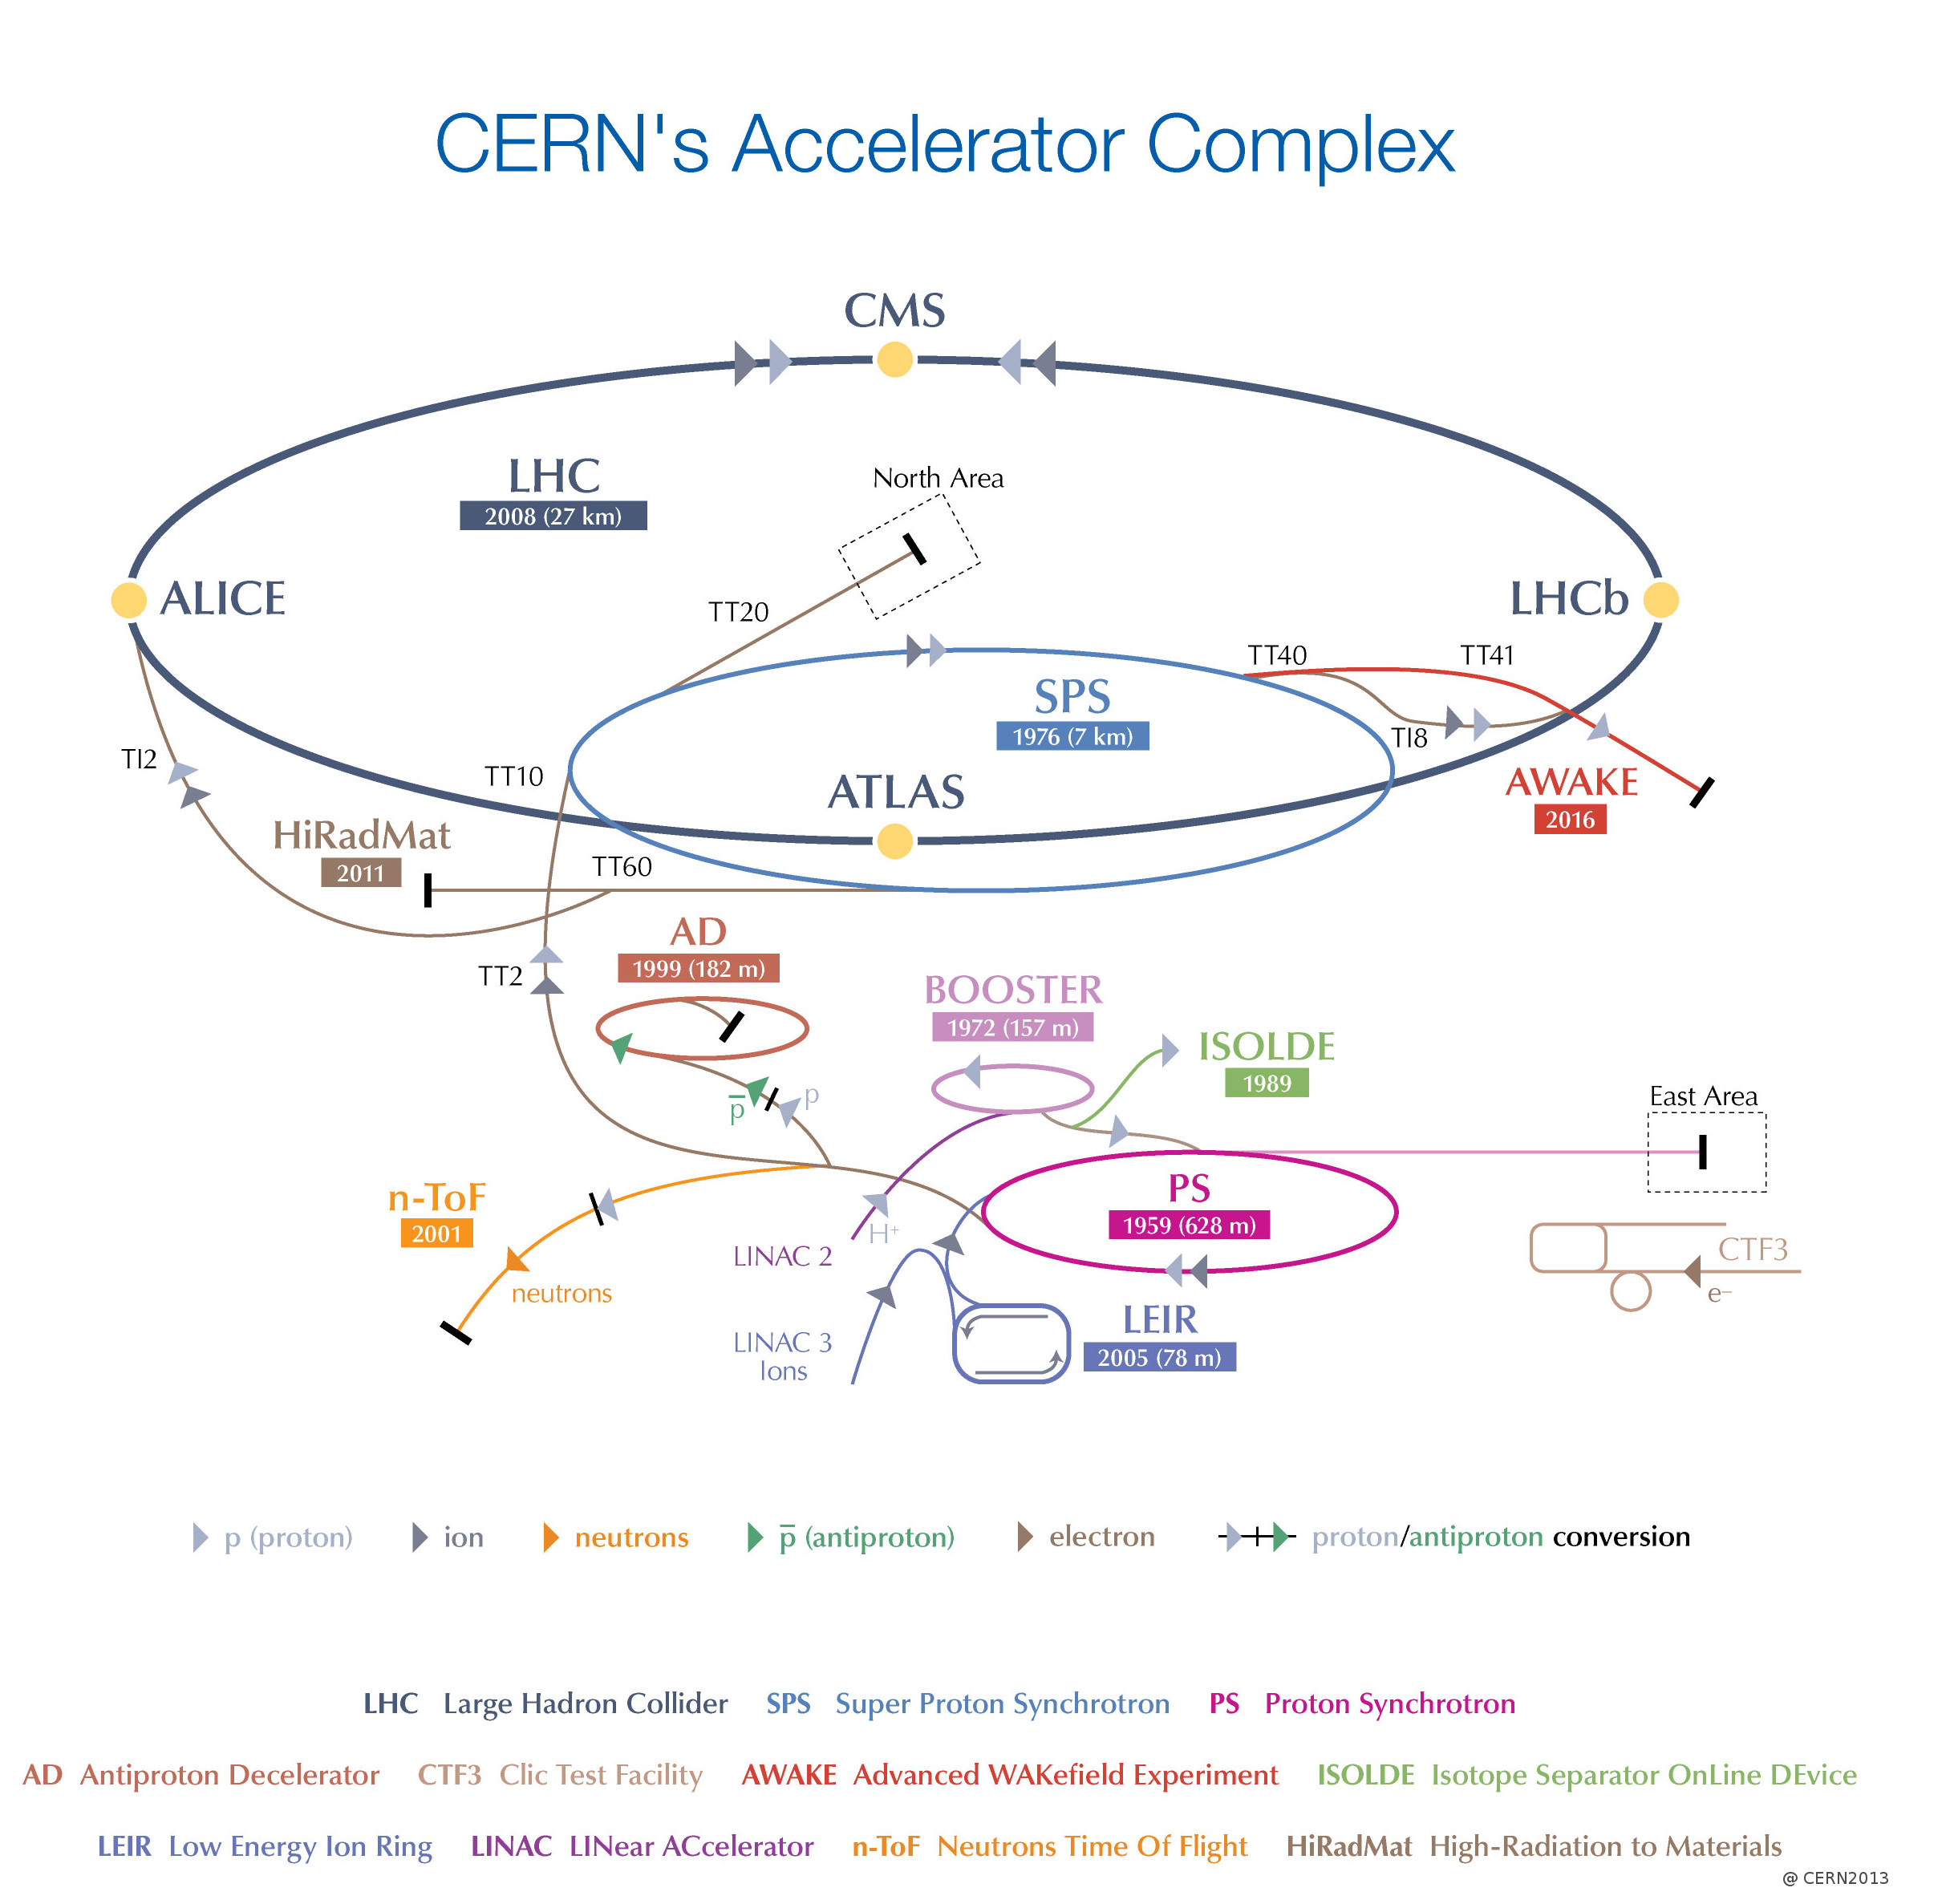
\includegraphics[width=0.98\textwidth]{../figs/Exp/CERN_accelerator_complex2013.jpg}}
    \caption{CERN's accelerator complex~\cite{ref_fig_CERNacceleratorComplex}.}
    \label{fig:CERN_accelerator_complex}
  \end{center}
\end{figure}

% brochure, page 15-17 - skip (19 of pdf doc)
% PLACE this sentence somewhere else; the rest of material is too basic

%brochure, page 18 (20 of pdf doc)

%brochure p 38 (42 of pdf doc) 
%Main goals of LHC were to detect the SM Higgs boson if it existed and to search for evidences of BSM physics which may give a clue on understanding the phenomena including but not limited to the dark matter, the matter-antimatter asymmetry, the nature of the gravitational force. 

Six detectors are installed at the LHC to detect products of hadron collisions and to perform measurements of the LHC physics program. There are general purpose detectors ATLAS and CMS, there is LHCb which specializes in the physics of B-mesons, and ALICE which is designed to detect products of heavy ion collisions. Also there are two relatively small detectors: LHCf and TOTEM which are installed close to the ATLAS and CMS collision points respectively. The greatest achievement by the LHC today is the discovery of the Higgs boson in~2012 by the CMS~\cite{ref_HiggsPaperCMS} and the ATLAS~\cite{ref_HiggsPaperATLAS} collaborations. 

%brochure 27 (31 of pdf doc)

%LHC is constructed of eight arcs, each arc corresponds to a sector as shown in Fig.~\ref{fig:LHCsectors}. In between there are eight insertions where beams are either collided or injected or dumped or cleaned. On the other hand, LHC is split on eight octants, each starting from the middle of one sector and ending at the middle of the next one. Thus, each octant includes one full insertion.\\ 

The design energy of the LHC is $\sqrt{s}=14$~TeV which corresponds to $14/2=7$~TeV per beam however it is taking years to reach the design energy, and, meanwhile, several lower energy points were and are being probed. In~2010-2011 the LHC operated at energy of~3.5~TeV per beam which was already higher than the energy of any other collider. In~2012 the energy increased up to~4~GeV. In~2013-2014 the LHC was shut down for upgrades. Collisions were restarted at~6.5~TeV in~2015 and continued at this energy in~2016. 

All critical measurements performed at lower energies are also repeated at higher energies because the ability to probe higher energy scales increases our chances for a discovery and even if no deviations from the known physics are found at a given energy point, the discovery is still possible to happen as we go higher in the energy. Precision SM measurements of cross section need to be done at all energies and compared to the theory since the cross sections evolve with energy. The cross sections of many interesting processes increase with energy because in a collision of higher energy hadrons more partons can participate in the interactions. Thus, rarer processes can be explored. Cross sections of various productions in $pp$ collisions and their energy dependencies are shown in Fig.~\ref{fig:LHC_totalCS}.

\begin{figure}
  \centering
  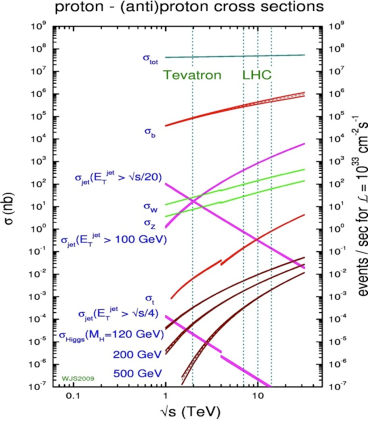
\includegraphics[width=.95\linewidth]{../figs/Exp/LHC_totalCS.png}
  \caption{Cross sections of of various productions in $pp$ collisions~\cite{ref_fig_LHC_totalCS}.}
  \label{fig:LHC_totalCS}
\end{figure}

%\begin{figure}
%  \centering
%  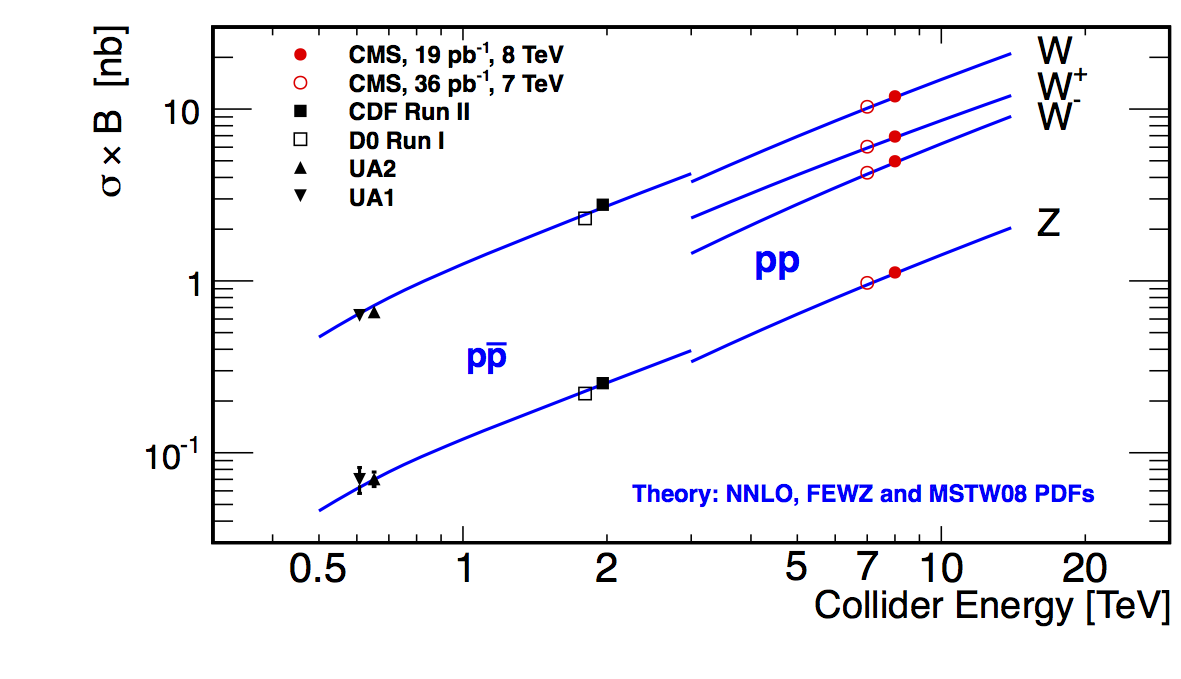
\includegraphics[width=.80\linewidth]{../figs/Exp/cms-sigma-vs-e.png}
%  \caption{Cross section of $W$ and $Z$ production in $pp$ collisions~\cite{ref_fig_LHC_CS_WandZ}.}
%  \label{fig:LHC_CS_WandZ}
%\end{figure}

%While different BSM searches have been constituting a significant part of the LHC physics program since the beginning of its operation, no deviations from the SM were found by any of the experiments. The searches continue with higher beam energies and larger amount of data.

In addition to the beam energy, there are many other collider parameters. A brief summary of them is available in Tab.~\ref{tab:LHCparameters}. One of the most critical parameters of an accelerator is the ability to produce a large number of interesting collisions which is determined by the luminosity (Ch.~\ref{sec:WgAbout_LumiAndCS}). The instantaneous luminosity is determined by the following expression~\cite{ref_PDG}:

\begin{equation}
L = f \frac{n_1 n_2}{4 \pi \sigma_x \sigma_y}
\end{equation}

\noindent{where $n_1$ and $n_2$ are numbers of particles in colliding bunches, $f$ is a frequency of collisions, $\sigma_x$ and $\sigma_y$ characterize sizes of overlapping parts of colliding beams in horizontal and vertical directions. Instantaneous luminosity multiplied by a cross section of a process gives an event rate (Eq.~\ref{eq:L_eventRate}). To determine the integrated luminosity, one has to integrate the instantaneous luminosity over time:}

\begin{equation}\label{eq:integratedL}
  L_{int}=\int L dt
\end{equation}

\noindent{With the integrated luminosity, one can compute the total number of events of interest over the full period of data taking. Thus the integrated luminosity of a data sample is a measure of the size of the data sample.}

The luminosity of the LHC is also higher than of any previously existed collider. The integrated luminosity of the LHC for $pp$ collisions for different years of the operation is shown in Fig.~\ref{fig:LHClumi}. Run periods of LHC in~2010-2012 refer to Run~I of the LHC operation. While working on the energy of $\sqrt{s}=7$~TeV, LHC delivered~45~pb$^{-1}$ and~6.1~fb$^{-1}$ of data in~2010 and~2011 year respectively. In~2012 the working energy of LHC was $\sqrt{s}=8$~TeV, and the integrated luminosity was $L_{int}=$23.3~fb$^{-1}$.  After a long shutdown, LHC was upgraded for Run~II, to operate on $\sqrt{s}=13$~TeV in~2015 and delivered~4.2~fb$^-1$ of data by the end of~2015. In~2016 LHC continued operating at $\sqrt{s}=13$~TeV and delivered the integrated luminosity of~41.1~fb$^{-1}$~\cite{ref_LHClumi_twiki}.

The measurement of this dissertation is performed at the energy of~4~TeV per beam or the center of mass energy $\sqrt{s}=8$~TeV with~19.6~fb$^{-1}$ of data. The same process was measured at $\sqrt{s}=7$~TeV with about four times less amount of data by both CMS and ATLAS. These measurements are discussed in greater details in Ch.~\ref{sec:WgAbout_PastMeas}.

% brochure page 30 (34 of pdf)
\begin{table}[h]
  \begin{center}
  \caption{ Main parameters of LHC~\cite{ref_LHC_brochure}}
  \vspace{5 mm}
  \begin{tabular}{|l|c|}
     \hline
     Circumference & 27 km  \\ \hline
     Dipole operating temperature &  1.9 K \\ \hline
     Number of magnets &  9593 \\ \hline
     Number of main dipoles &  1232 \\ \hline
     Number of main quadrupoles &  392 \\ \hline
     Number of RF cavities &  8 per beam \\ \hline
     Nominal energy, protons &  7 TeV \\ \hline
     Nominal energy, lead ions &  2.76 TeV per nucleon \\ \hline
     Peak magnetic dipole field &  8.33 T \\ \hline
     Min. distance between bunches &  7 m \\ \hline
     Design luminosity &  $10^{34}$ cm$^{-2}$ s$^{-1}$ \\ \hline
     No. of bunches per proton beam &  2808 \\ \hline
     No. of protons per bunch (at start) &  $1.1\times 10{11}$ \\ \hline
     No. of collisions per second &  600 millions \\ \hline
  \end{tabular}
  \label{tab:LHCparameters}
  \end{center}
\end{table}

\begin{figure}
  \centering
  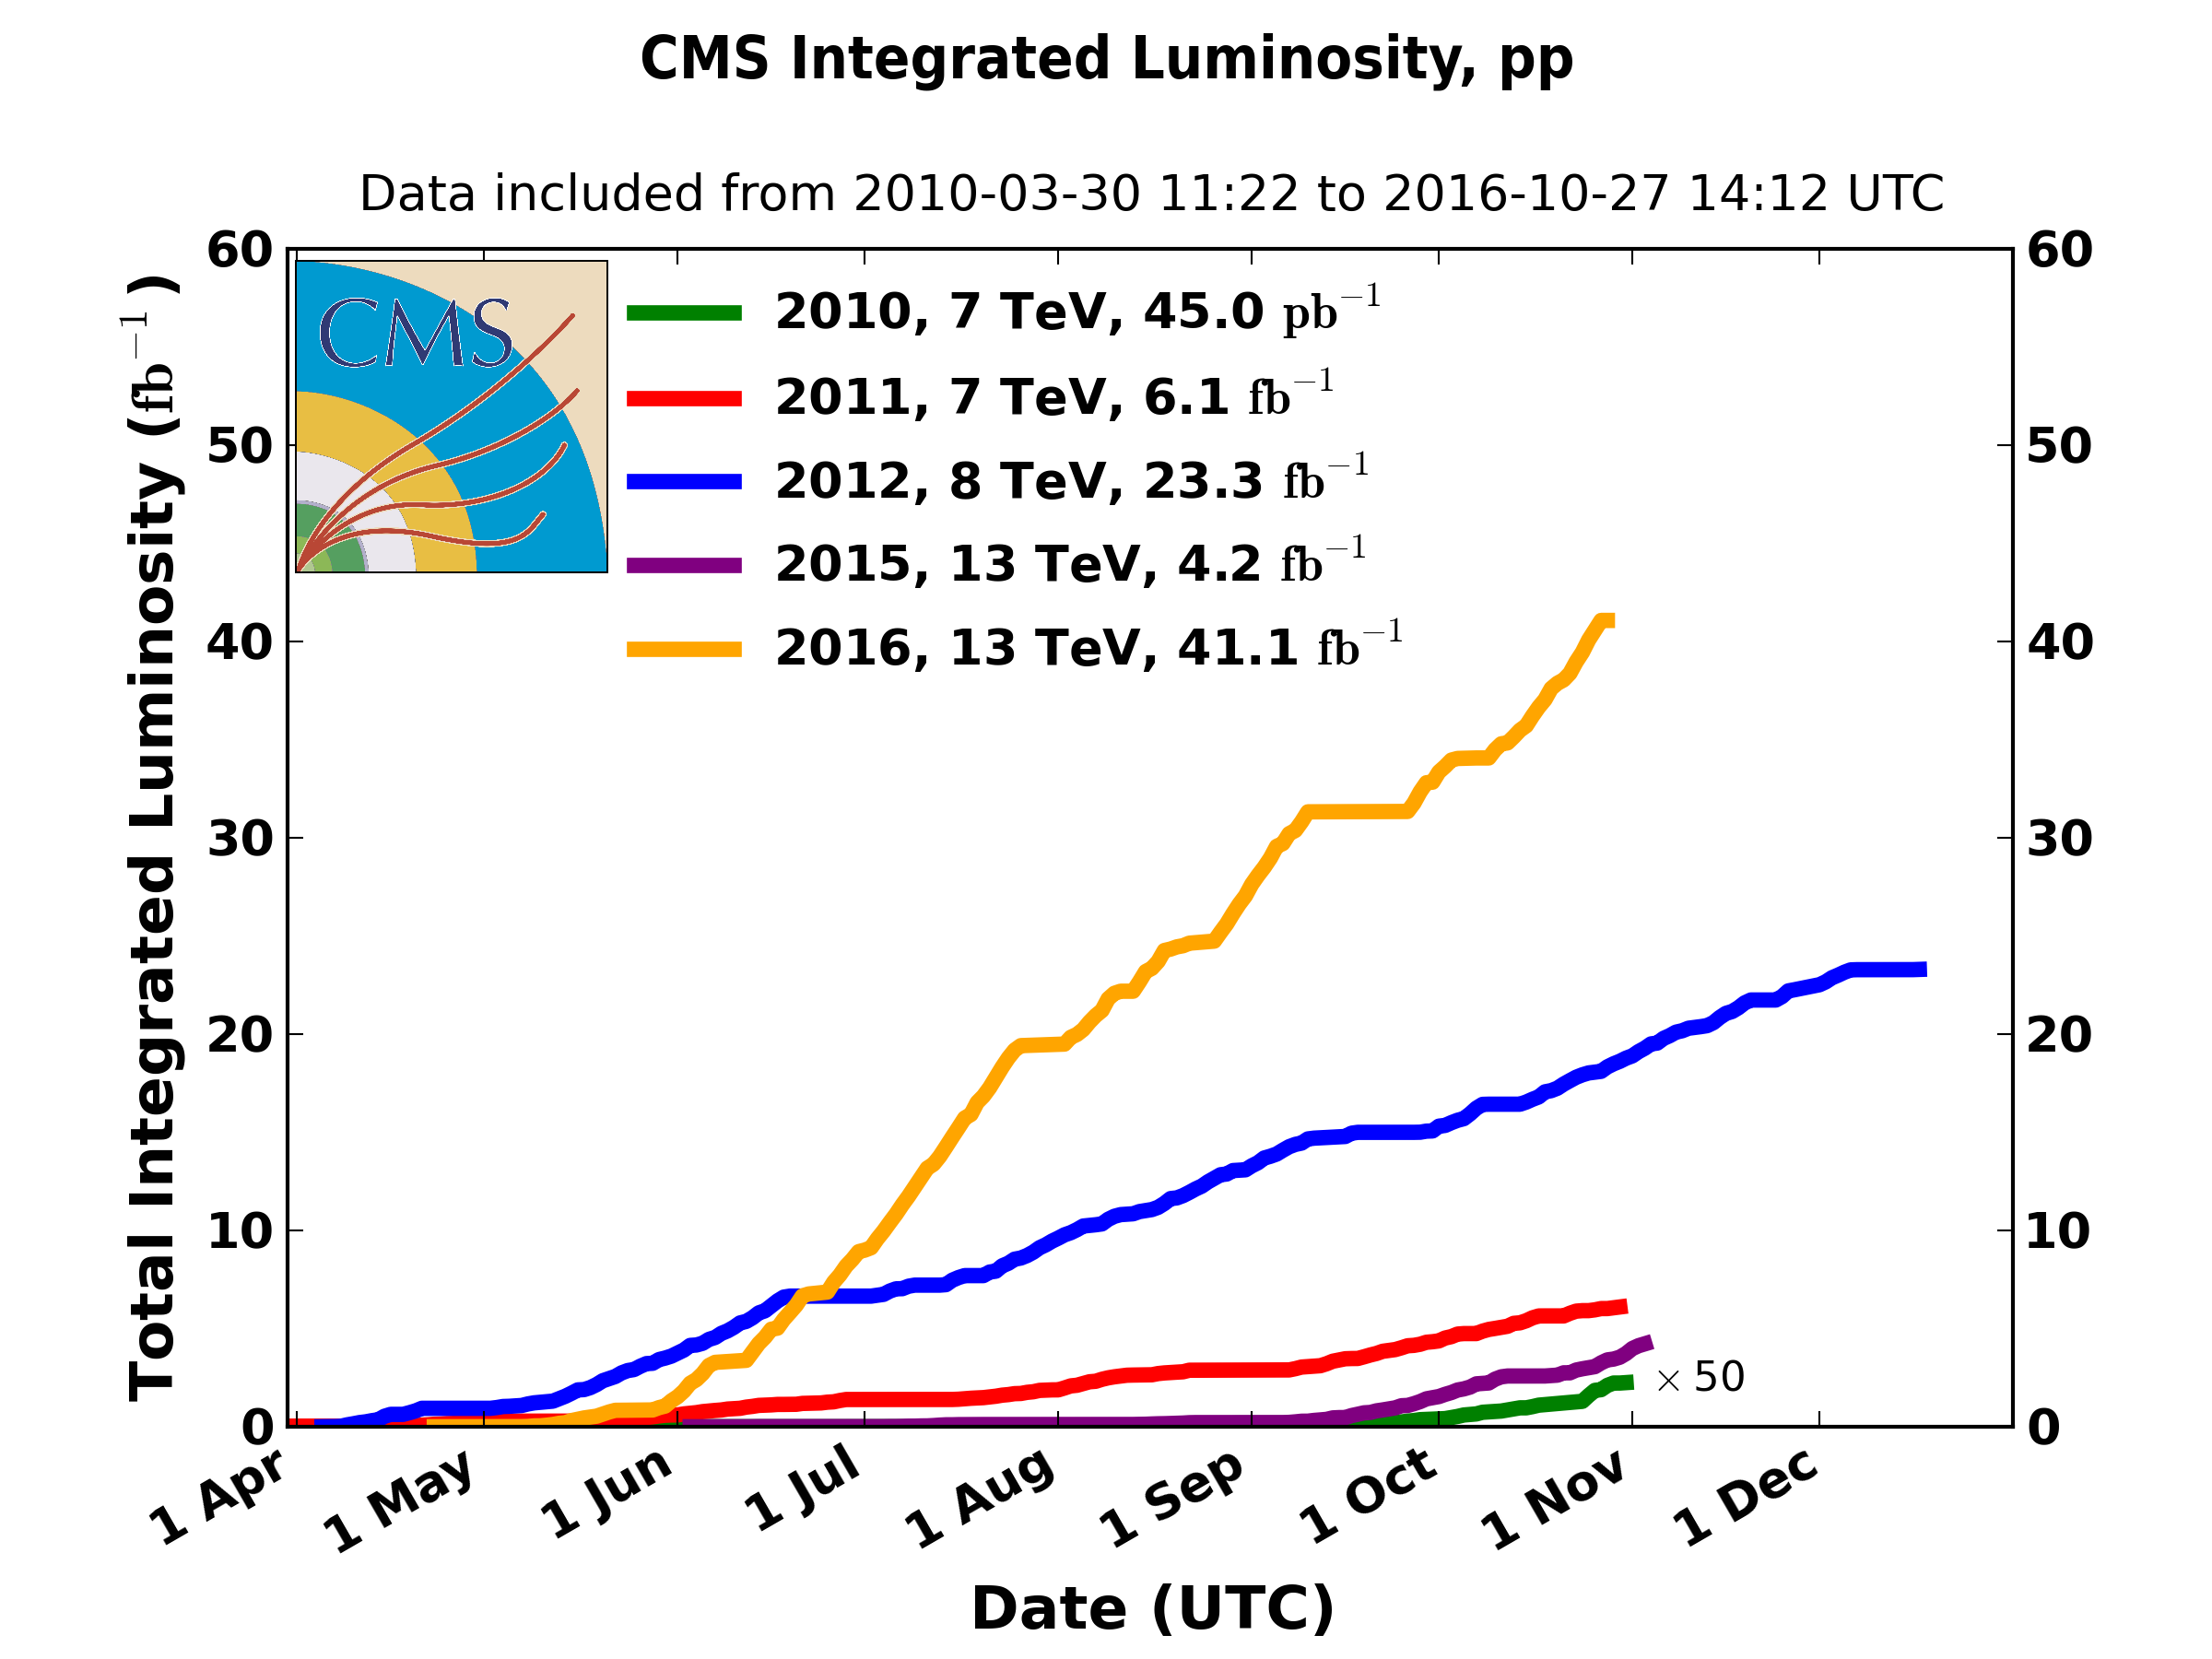
\includegraphics[width=.80\linewidth]{../figs/Exp/int_lumi_cumulative_pp_2.png}
  \caption{LHC integrated luminosity by year~\cite{ref_fig_LHClumi}.}
  \label{fig:LHClumi}
\end{figure}

% begin: LHC lumi and LHC sectors
%\begin{figure}
%\centering
%\begin{minipage}{.48\textwidth}
%  \centering
%  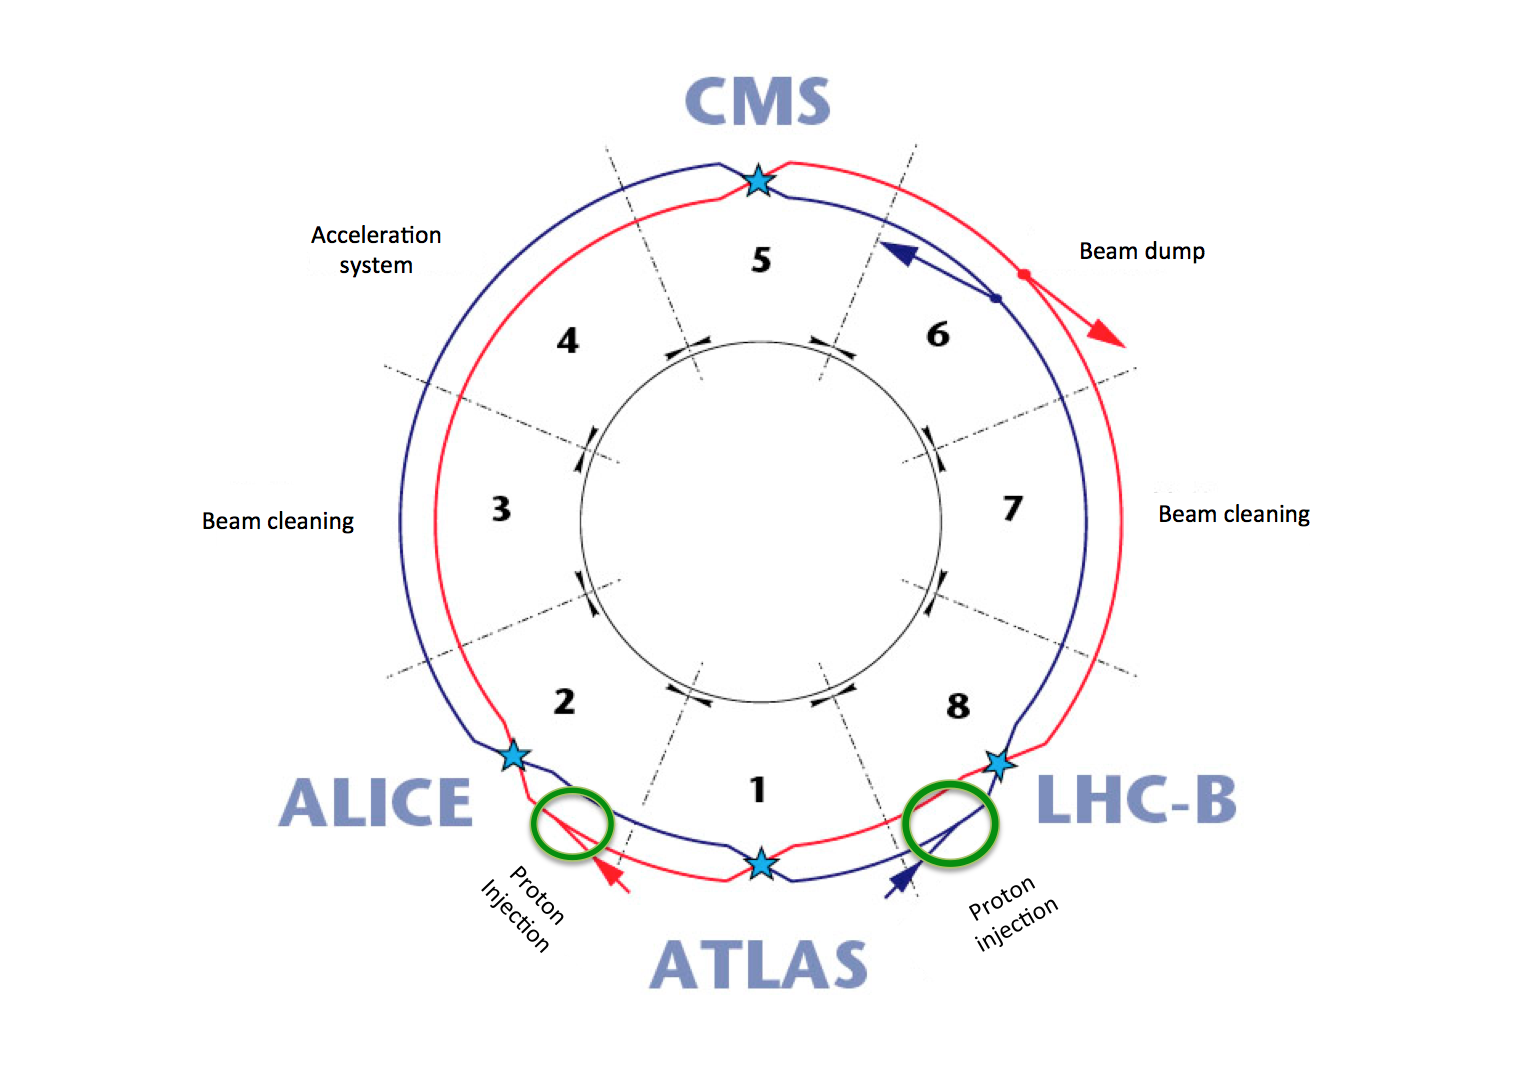
\includegraphics[width=.95\linewidth]{../figs/Exp/LHC_sectors.png}
%  \caption{Schematic view of LHC sectors. Source of the figure: \cite{ref_fig_LHCsectors}.}
%  \label{fig:LHCsectors}
%\end{minipage}%
%\begin{minipage}{.48\textwidth}
%  \centering
%  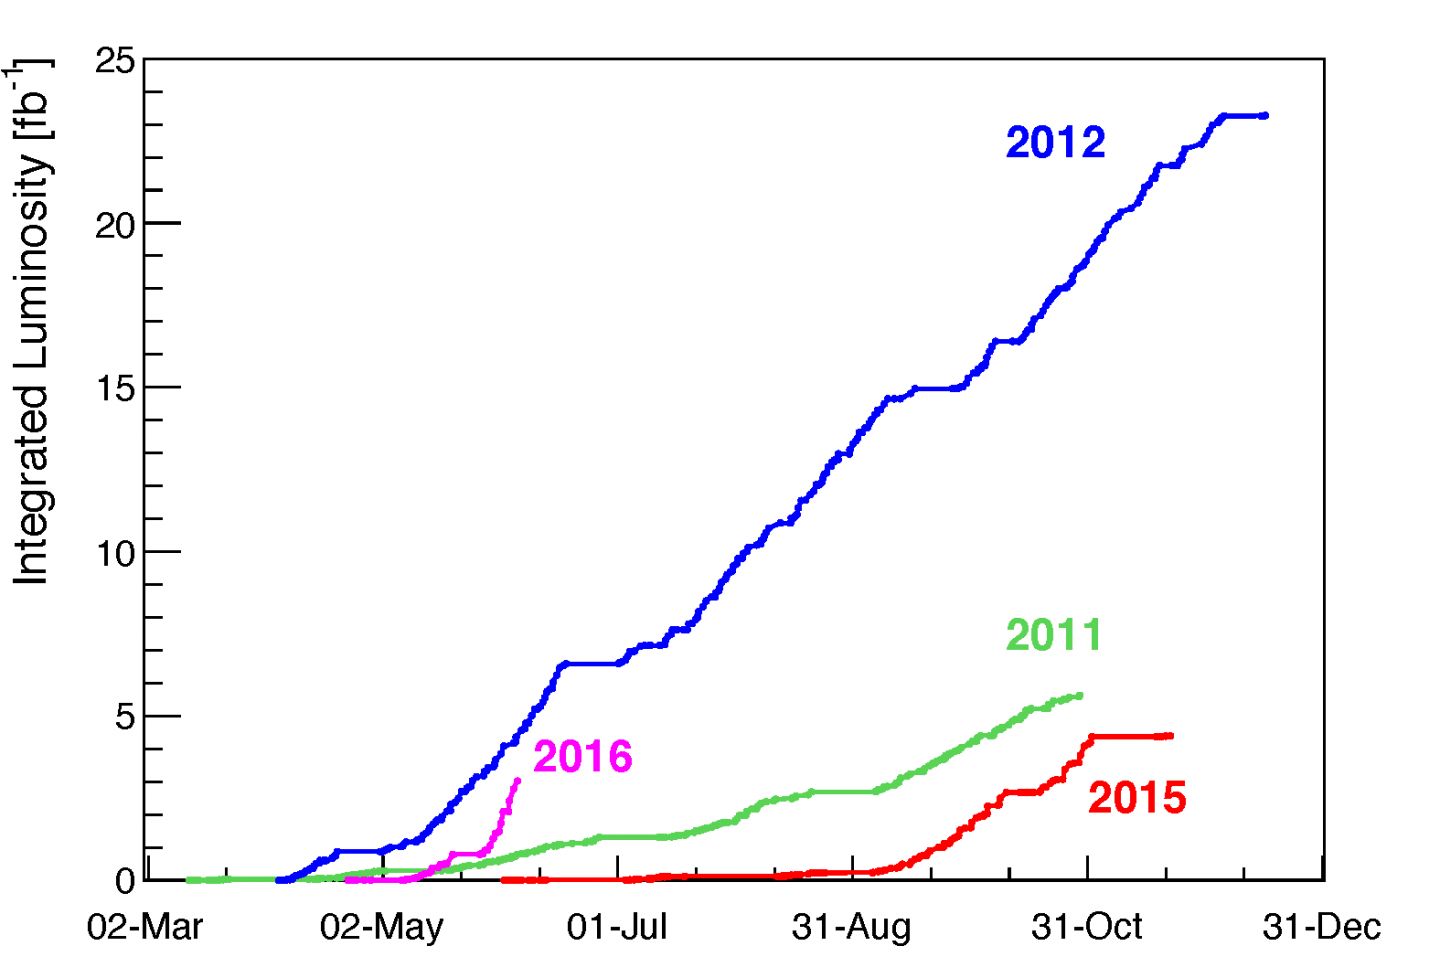
\includegraphics[width=.95\linewidth]{../figs/Exp/LHC_lumi.png}
%  \caption{LHC integrated luminosity by year. Source of the figure: \cite{ref_fig_LHClumi}.}
%  \label{fig:LHClumi}
%\end{minipage}
%\end{figure}
% end: LHC lumi and LHC sectors
